\chapter{Use Cases}

\section{Avoiding Class Name Clashes}
\begin{wrapfigure}{l}{0.55\textwidth}
	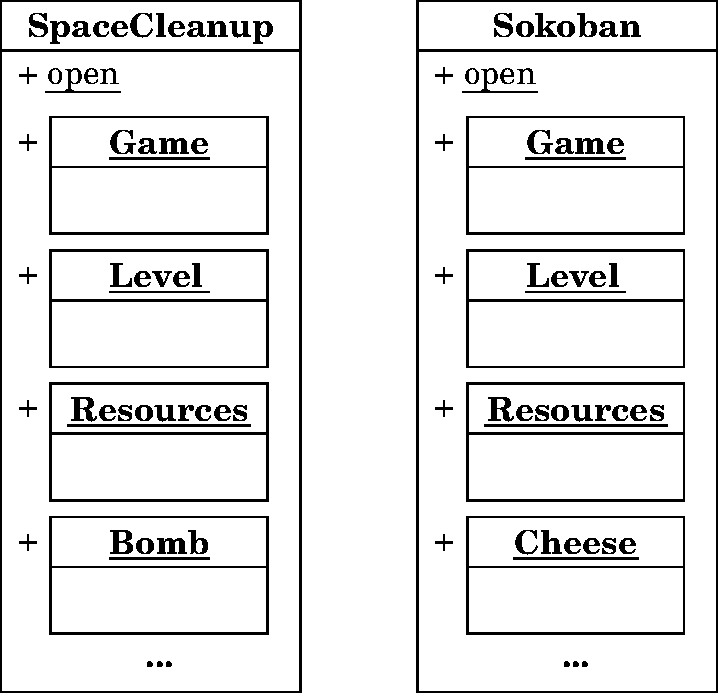
\includegraphics[width=0.5\textwidth]{usecase_class_clash.pdf}
	\centering
	\caption{Resolving class name clashes with class nesting}
	\label{fig:use_class_clash}
\end{wrapfigure}

In this example, class nesting is used to avoid class name clashes and to give every class a unique fully qualified name. Consider, that we want two load two computer games in a single Squeak image. The first game is a bomberman game, providing classes \texttt{Game}, \texttt{Level}, \texttt{Resources} among others. The second game is a Sokoban game, and has three classes with the same name. Without our system, this would be a problem: as soon as another class with the same is installed, the old one is overwritten with the new name.

With our system, two classes with the same name can coexist in the same image, as long as they are nested within different classes (Figure~\ref{fig:use_class_clash}).

Note, that, for example, \texttt{Bomberman Game} and \texttt{Sokoban Game} are different classes. Whenever a class inside \texttt{Bomberman} references \texttt{Game} using the source code statement \texttt{scope Game} or \texttt{Game} (equivalent statement), the method lookup recurses in the enclosing classes, until \texttt{Game} is found in the \texttt{Bomberman} class.

\section{Module Versioning and Dependency Management}
In this example, class nested is used to keep multiple different versions of the same library in one image. This is necessary if two applications require different versions of the same library. In the best case, the API of a library should not change within one major version, such that a newer library version should work with an application that was developed with an older library version. However, sometimes, application developers have to work around known bugs or rely on implementation-specific classes which are not designed to be used by library users and subject to change. In that case, application code can break when suddenly a different version of the library is used.

\subsection{Representing Module Versions}
\begin{wrapfigure}{l}{0.55\textwidth}
	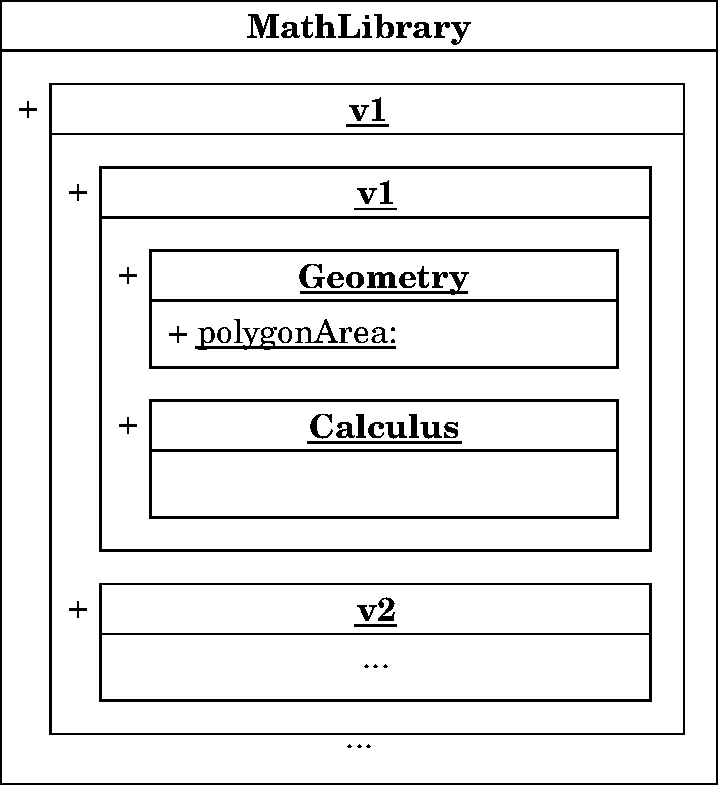
\includegraphics[width=0.5\textwidth]{usecase_define_version.pdf}
	\centering
	\caption{Module versioning}
	\label{fig:use_module_ver}
\end{wrapfigure}

Figure~\ref{fig:use_module_ver} shows how nested classes can be used for module versioning. In this example, we are developing a library for mathematical operations. The top-level class contains nested classes for every major version. Every major version can again have nested classes for minor versioning. In fact, this scheme can be used to have any kind of versioning system, as long as it is based in numbers.

Two versions of \texttt{MathLibrary} are installed in this example: version 1.1 and version 1.2. These versions can be referenced by writing \texttt{MathLibrary v1 v1} and \texttt{MathLibrary v1 v2}. Note, that even though all versions define classes with the same name, no class clashes occur. If a class in \texttt{MathLibrary} references another class in \texttt{MathLibrary}, the method lookup will look for classes in the same version of \texttt{MathLibrary}.

\subsection{Aliasing Module Versions}
Whenever an application requires a class from a library in a certain version, the application can either write down the fully qualified name of the class or create an alias. For example, the fully qualified name of the class \texttt{Calculus} in \texttt{MathLibrary} version 1.2 is \texttt{MathLibrary v1 v2 Calculus}. However, it is very likely that an application requires more than just one class from a library. In this case, an alias should be defined, because it keeps the required version number at a single point in the code (making it easy to change the version) and results in less verbose code.

\begin{figure}[!htp]
\begin{lstlisting}
<@\textbf{MyApplication>>MathLibrary}@>
    ^ Repository MathLibrary v1 v2

<@\textbf{MyApplication>>rectArea:}@> origin <@\textbf{extent:}@> extent
    ^ MathLibrary polygonArea: { 
        origin x @ origin y.
        (origin x + extent x) @ y.
        (origin x + extent x) @ (origin y + extent y).
        origin x @ (origin y + extent y) }
\end{lstlisting}
\caption{Defining class aliases}
\label{fig:use_alias}
\end{figure}

Figure~\ref{fig:use_alias} shows how class alias can be used to specify module versions at a single point in the code. The programmers defines a method\texttt{MathLibrary} returning the module in the required version. In \texttt{MyApplication>>rectArea:extent:}, the reference to \texttt{MathLibrary} will be replaced with \texttt{scope MathLibrary}, which will call the aliased method. Note, that in \texttt{MyApplication>>MathLibrary}, we have to reference the library with \texttt{Repository MathLibrary}, forcing the lookup to start at the root of our system. Otherwise, the method \texttt{MathLibrary} would call itself.

\paragraph{Helper Methods}
In Figure~\ref{fig:use_module_ver} the top-level class and major version should be a subclass of the class \texttt{Versioning}, a class provided by our system. This class contains convenience methods making it easier to work with version containers. The following list gives an overview of the helper methods \texttt{Versioning} provides.

\begin{itemize}
	\item \texttt{Versioning>>myLatest}: returns the latest version contained as a nested class in the receiver. For example, \texttt{MathLibrary myLatest} returns \texttt{MathLibrary v1}.
	\item \texttt{Versioning>>latest}: returns the lastest version in the receiver recursively. For example, \texttt{MathLibrary latest} returns \texttt{MathLibrary v1 v2}.
	\item \texttt{Versioning>>atLeast:}: returns the latest version recursively and asserts that its version number is greater than the parameter. For example, \texttt{MathLibrary atLeast: '1.1'} returns \texttt{MathLibrary v1 v2}, and \texttt{MathLibrary atLeast: '1.3'} throws an error.
\end{itemize}

\subsection{External Configuration}
Parameterized classes can not only be used to build mixins, but also externally configuarable modules. The basic idea is taken from Newspeak, where all module dependencies are encapsulated in a \texttt{platform} object. This platform object is installed along with the application source code and contains all libraries that the application depends on in the correct version~\cite{bracha2008newspeak}. This has the advantage that there is no need for a global namespace and all references to external classes are resolved using the platform object, effectively making import statements obsolete. A configurable module does not need to know anything about concrete implementations of external libraries, as long as the implementations provided in the platform implement the expected interfaces.

In our system, methods inside parameterized classes can reference arguments provided to the class accessor method. The idea is that, instead of referencing classes in the global namespace, the programmer references these arguments. The user of the module can then decide which exact implementation he wants to use.

\paragraph{Example}
Figure~\ref{fig:use_paintbrush} shows part of the implementation of simple drawing application. \texttt{PaintbrushWith:IO:} is a parameterized top-level class which takes as arguments a matrix implementation and a file IO library. The matrix implementation is used for storing the pixels inside the application. In the simplest case, this is could be the class \texttt{Matrix} from the Squeak standard library. It could, however, also be a class which stores pixels in a compressed form (e.g., using run-length encoding), but has \texttt{at:}, \texttt{at:put:}, \texttt{rows}, and \texttt{columns} as public API methods. \texttt{ReaderWriter} must be a class or object that supports reading and writing files on a pixel-by-pixel basis. Depending on which IO class the user of the library provides to \texttt{PaintbrushWith:IO:}, the application might for example generate JPEG files or PNG files.

\begin{figure}[!htp]
\centering
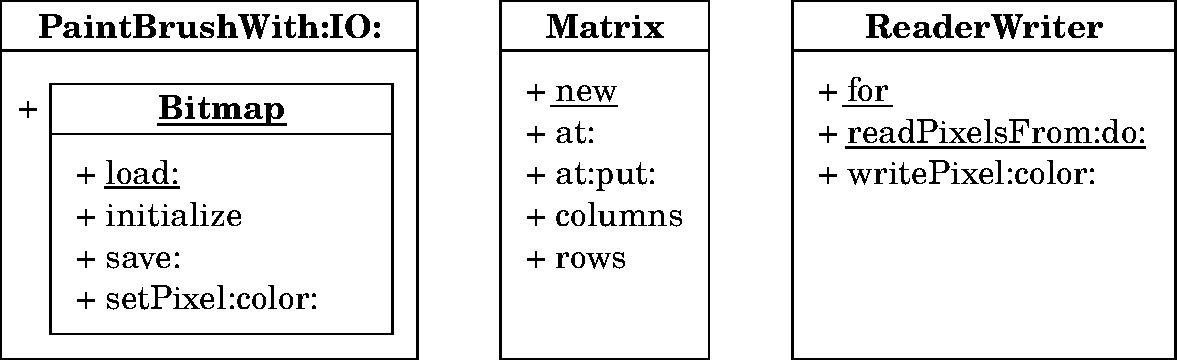
\includegraphics[width=0.8\textwidth]{usecase_paintbrush.pdf}

\begin{lstlisting}
<@\textbf{PaintbrushWith:}@> Matrix <@\textbf{IO:}@> ReaderWriter
    <@\textcolor{OliveGreen}{\textbf{< class >}}@>
    ^ Object subclass

<@\textbf{(PaintbrushWith:}@> Matrix <@\textbf{IO:}@> ReaderWriter<@\textbf{) class>>Bitmap}@>
    <@\textcolor{OliveGreen}{\textbf{< class >}}@>
    ^ Object subclassWithInstVars: <@\textcolor{RoyalPurple}{'pixels'}@>

<@\textbf{(PaintbrushWith:}@> Matrix <@\textbf{IO:}@> ReaderWriter<@\textbf{) class>>Bitmap>>initialize}@>
    pixels := Matrix new.

<@\textbf{(PaintbrushWith:}@> Matrix <@\textbf{IO:}@> ReaderWriter<@\textbf{) class>>Bitmap>>}@>
        <@\textbf{setPixel:}@> aPoint <@\textbf{color:}@> aColor
    pixels at: aPoint put: aColor.

<@\textbf{(PaintbrushWith:}@> Matrix <@\textbf{IO:}@> ReaderWriter<@\textbf{) class>>Bitmap class>>}@>
        <@\textbf{load:}@> aFile
    <@\textcolor{Gray}{| instance |}@>
    <@\textcolor{Gray}{instance}@> := self new.
    ReaderWriter 
        readPixelsFrom: aFile
        do: [ :point :color | <@\textcolor{Gray}{instance}@> setPixel: point color: color ].
    ^ <@\textcolor{Gray}{instance}@>

<@\textbf{(PaintbrushWith:}@> Matrix <@\textbf{IO:}@> ReaderWriter<@\textbf{) class>>Bitmap>>save:}@> aFile
    <@\textcolor{Gray}{| writer |}@>
    <@\textcolor{Gray}{writer}@> := ReaderWriter BitmapWriter for: aFile.
    1 to: pixels columns do: [ :x |
        1 to: pixels rows do: [ :y | 
            <@\textcolor{Gray}{writer}@> writePixel: x@y color: (pixels at: x@y) ] ].
    <@\textcolor{Gray}{writer}@> close.
\end{lstlisting}
\caption{Parameterized classes for external module configuration}
\label{fig:use_paintbrush}
\end{figure}

It is important to understand that the implementation of \texttt{PaintbrushWith:IO:} is entirely decoupled from the pixel data structure representation and the import/export functionality. It is up to the user of \texttt{PaintbrushWith:IO:} to configure the class as needed.

\subsection{Dependency Injection}




\section{Readability and Understandability}
example: large project, where parts of the code can now be understood, given that we have hierarchical nesting. could be an example where grouping according to multiple criteria is needed (would result in n x m packages)

\section{Mixin Modularity with Parameterized Classes}

\section{Class Generator Pattern}
\label{sec:usecase_classgen}
better syntax for class generators

\section{Extension Methods}
better way is needed (e.g., class boxes, refinements, COP, world (paper viewpoints), monkey patching). return already existing class in generator method
